% !TEX program = pdflatex
\documentclass[letterpaper, 10pt, conference]{IEEEtran}

\usepackage{amsmath,amssymb,amsfonts}
\usepackage{amsthm}
\usepackage{algorithmic}
\usepackage{algorithm}
\usepackage{graphicx}
\usepackage{textcomp}
\usepackage{booktabs}
\usepackage{multirow}
\usepackage{cite}
\usepackage{hyperref}
\usepackage{xcolor}
\usepackage{bm}
\usepackage{tikz}
\usetikzlibrary{arrows.meta,positioning,calc,shapes.geometric,fit,backgrounds}

% Compact lists
\usepackage{enumitem}
\setlist{nosep}

% Theorem environments
\newtheorem{definition}{Definition}
\newtheorem{proposition}{Proposition}
\newtheorem{theorem}{Theorem}
\newtheorem{remark}{Remark}

% Math shortcuts
\newcommand{\R}{\mathbb{R}}
\newcommand{\Spp}{\mathbb{S}_{++}}
\newcommand{\balpha}{\bm{\alpha}}
\newcommand{\bx}{\bm{x}}
\newcommand{\bu}{\bm{u}}
\newcommand{\bq}{\bm{q}}
\newcommand{\bp}{\bm{p}}
\newcommand{\bK}{\bm{K}}
\newcommand{\bone}{\mathbbm{1}}
\newcommand{\cW}{\mathcal{W}}
\newcommand{\cS}{\mathcal{S}}
\newcommand{\cI}{\mathcal{I}}
\newcommand{\cX}{\mathcal{X}}
\newcommand{\cU}{\mathcal{U}}
\newcommand{\bs}{\bm{s}}

\begin{document}

\title{Template MPC for Switched LPV Robotic Systems:\\
  Learned Contact Scheduling with Structured Dynamics}

\author{
  \IEEEauthorblockN{Jianghan Zhang}
  \IEEEauthorblockA{Dartmouth College\\
  \texttt{jianghan.zhang.gr@dartmouth.edu}}
}

\maketitle

% ================================================================
\begin{abstract}
We present a four-layer control architecture for legged robots
in which the \emph{only} external specification is a six-dimensional
body-pose command (position and orientation of the center of mass
relative to the support polygon).
From this command, the system autonomously determines
where to place its feet, what dynamics govern each contact phase,
and what joint torques to apply---with no pre-defined gait table
and no analytical dynamics model.

The four layers are:
(i)~a \emph{user command} $\bm{s} \in \R^6$
  specifying the desired body pose;
(ii)~a \emph{Footstep Planner Network} that maps the command
  and current state to a time-stepped sequence of desired
  end-effector positions over the MPC horizon, from which
  the contact mode at each timestep is derived via the
  signed distance to the contact surface;
(iii)~per-mode \emph{Euler--Lagrangian Networks} (EL-Nets) that
  provide smooth linearized dynamics while preserving
  symmetric positive-definite inertia, energy conservation,
  and passivity;
and (iv)~a \emph{DARE-cached MPC solver} that assembles a
  complete time-varying quadratic program from these pieces
  and solves it via precomputed Riccati gains.

The MPC problem is not passed through a monolithic solver;
it is \emph{assembled} at each timestep from four independently
sourced components: the reference (from the user command),
the contact constraints and scheduling variable (from the Planner),
the dynamics matrices (from the EL-Nets), and the feedback
gains (from the DARE cache).
This generalizes the flat-parameterized TinyMPC
framework~\cite{zhang2025flat} from quadrotors
(single mode, analytic dynamics) to switched linear
parameter-varying (LPV) systems with learned dynamics
and learned contact scheduling.
\end{abstract}

% ================================================================
\section{Introduction}\label{sec:intro}

Model-predictive control (MPC) is a central tool for controlling
robots subject to state and input constraints~\cite{tinympc}.
For systems with persistent contacts---such as quadrupedal
locomotion---the dominant paradigm is \emph{whole-body control}
(WBC)~\cite{kim2019}: a pre-defined gait scheduler selects
the contact sequence, and a quadratic program computes joint
torques that respect contact constraints, friction cones,
and dynamic feasibility.
The MIT Cheetah~\cite{kim2019} and similar platforms demonstrate
the effectiveness of this approach at moderate speeds with
analytical rigid-body dynamics.

Two limitations of the standard WBC pipeline motivate our work.
First, the contact sequence is \emph{pre-defined}---typically
a periodic gait table (trot, bound, gallop)---which prevents
reactive adaptation to unstructured terrain.
Second, the dynamics model is \emph{analytical}, requiring
accurate knowledge of inertial parameters, joint friction,
and contact geometry.
For complex morphologies or soft contacts, such models are
difficult to obtain.

In prior work~\cite{zhang2025flat}, we showed that for quadrotors---a
contact-free, differentially flat system---the DARE solution
can be cached over a four-dimensional flat parameter
$\balpha = (a_x, a_y, a_z, \psi)$,
reducing online MPC to ${\sim}260$ arithmetic operations.
The key enabler was that differential flatness compresses the
scheduling variable from $\R^n$ to $\R^4$.

This paper generalizes the construction to \emph{switched
linear parameter-varying} (LPV) systems---the natural abstraction
for robots that make and break contacts.
We propose a four-layer architecture in which each layer has
exactly one responsibility and one mathematical type:

\begin{center}
\small
\begin{tabular}{@{}clp{1.6cm}p{2.2cm}@{}}
\toprule
Layer & Role & Input & Output \\
\midrule
1. Command & Intention & --- & $\bm{s} {\in} \R^6$ \\
2. Planner & Foot placement & $\bx, \bm{s}, \cS$ &
  $\bp^{\mathrm{des}}_i(t)$ \\
3. MPC & Torques & $\sigma, \balpha, \bx$ &
  $\bm{\tau} {\in} \R^m$ \\
4. Low-level & Execution & $\bm{\tau}$ & motor cmds \\
\bottomrule
\end{tabular}
\end{center}

Each layer \emph{reduces} the problem:
$6$ numbers of intention $\to$
$C \times 3 \times N$ numbers of contact geometry $\to$
$m$ numbers of torques $\to$ hardware.
No layer crosses the smooth/nonsmooth boundary:
the Footstep Planner (Layer~2) handles all discrete contact
decisions; the MPC solver (Layer~3) sees only smooth dynamics.

The architecture mirrors the whole-body control (WBC)
pipeline~\cite{kim2019} but replaces its two pre-specified
components:

\begin{center}
\small
\begin{tabular}{@{}lcc@{}}
\toprule
Component & WBC~\cite{kim2019} & Ours \\
\midrule
User input       & Body-pose cmd   & Same \\
Contact sched.   & Pre-defined gait    & Learned \\
Dynamics         & Analytical RBD      & EL-Net \\
Feedback         & QP (online)         & DARE (offline) \\
Pre-specif.      & Gait + dynamics    & \textbf{Nothing} \\
\bottomrule
\end{tabular}
\end{center}

\noindent
The only external input is the user's body-pose command
$\bm{s} \in \R^6$---six numbers.
Everything else is either learned (Footstep Planner, EL-Net)
or derived from classical control theory (DARE cache).
Pre-defined gaits (trot, walk, gallop) can serve as a
bootstrapping curriculum for training the Footstep Planner,
enabling a smooth transition from classical to learned scheduling.

\subsection*{Contributions}
\begin{enumerate}
  \item A \emph{four-layer architecture} (user command $\to$
    footstep planner $\to$ smooth MPC $\to$ low-level control)
    in which the only external specification is a six-dimensional
    body-pose command.
    The MPC problem at each timestep is \emph{assembled}---not
    passed through a monolithic solver---from four independently
    sourced components: reference, contact schedule, dynamics,
    and feedback gains (Section~\ref{sec:architecture}).
  \item A \emph{switched LPV} formulation with precise geometric
    primitives (world frame, contact surface, signed distance),
    contact modes as derived quantities, and a scheduling variable
    that is exactly determined by the relative contact geometry
    (Section~\ref{sec:formulation}).
  \item A \emph{Footstep Planner Network} that outputs a
    time-stepped sequence of desired end-effector positions
    over the MPC horizon, from which per-timestep contact modes
    are derived---enabling time-varying mode sequences within
    a single predictive horizon (Section~\ref{sec:footstep}).
  \item \emph{EL-Nets}: Euler--Lagrangian structured neural networks
    for per-mode dynamics with guaranteed SPD inertia, energy
    conservation, and passivity.
    Gravitational potential is analytically known; only internal
    potentials are learned (Section~\ref{sec:elnet}).
  \item A generalized equivalence chain (Theorem~\ref{thm:chain})
    and sufficient conditions (Proposition~\ref{prop:conditions}),
    with the quadrotor result of~\cite{zhang2025flat} recovered
    as a single-mode special case (Section~\ref{sec:analysis}).
\end{enumerate}

% ================================================================
\section{Problem Formulation}\label{sec:formulation}

\subsection{Geometric Primitives}\label{sec:geometry}

We begin by establishing the geometric objects needed to define
contacts.

\begin{definition}[World Frame and Contact Surface]\label{def:geometry}
A \emph{world frame} $\cW$ is an inertial reference frame
with a distinguished ``up'' direction $e_z$.
The \emph{gravity vector} is $\bm{g} = -g \, e_z \in \R^3$
with $g > 0$.
A \emph{contact surface} $\cS$ is a subset of $\cW$
represented by a signed distance function
$\phi : \R^3 \to \R$, with $\cS = \{\bp \in \R^3 : \phi(\bp) = 0\}$
and $\phi(\bp) > 0$ for points above $\cS$.
\end{definition}

For flat ground, $\phi(\bp) = p_z$ and $\cS = \{p_z = 0\}$.
For general terrain, $\phi$ is a signed distance field (SDF)
that may be provided by a depth sensor or terrain map.

\begin{definition}[Contact Points and Contact Mode]\label{def:contact}
A robot has $C$ \emph{potential contact points}
(e.g., feet, fingertips) whose positions in $\cW$ are
functions of the generalized coordinates:
$\bp_i(\bq) \in \R^3$, $i = 1, \ldots, C$.
The \emph{contact mode} is the binary vector
\begin{equation}\label{eq:sigma}
  \sigma \in \{0,1\}^C, \quad
  \sigma_i = \begin{cases}
    1 & \text{if } \phi(\bp_i(\bq)) = 0, \\
    0 & \text{if } \phi(\bp_i(\bq)) > 0.
  \end{cases}
\end{equation}
The set of \emph{reachable modes} is
$\cI \subseteq \{0,1\}^C$ with $|\cI| \leq 2^C$.
\end{definition}

\begin{remark}[Contact Mode Is Derived, Not Prescribed]
\label{rem:derived}
The contact mode $\sigma$ is a \emph{consequence} of
the end-effector positions relative to $\cS$,
not an independent control input.
To break contact $i$, one moves $\bp_i$ so that
$\phi(\bp_i) > 0$; to make contact, one moves $\bp_i$
onto $\cS$.
This observation motivates the Footstep Planner architecture
in Section~\ref{sec:footstep}.
\end{remark}

\subsection{Robot State Decomposition}\label{sec:decomposition}

We decompose the robot state into three components,
each with a distinct role in the scheduling variable.

\begin{definition}[State Decomposition]\label{def:decomp}
The robot state is partitioned as
\begin{equation}\label{eq:decomp}
  \bx = (\bx_{\mathrm{com}},\; \bx_{\mathrm{ee}},\; \cW),
\end{equation}
where:
\begin{enumerate}
  \item $\bx_{\mathrm{com}}$ is the \emph{center-of-mass (COM) state}:
    position, velocity, orientation, and angular velocity of the
    floating base, expressed in $\cW$.
  \item $\bx_{\mathrm{ee}} = (\bp_1, \ldots, \bp_C)$ is the
    \emph{end-effector configuration}: positions of all $C$
    potential contact points in $\cW$.
  \item $\cW$ provides the gravity vector $\bm{g}$ and the
    contact surface $\cS$.
\end{enumerate}
\end{definition}

The absolute COM position in $\cW$ does not affect the
linearized dynamics (by translational invariance of the
equations of motion).
What matters is the \emph{relative geometry}:

\begin{definition}[Scheduling Variable]\label{def:alpha}
For a given contact mode $\sigma$, the \emph{scheduling variable}
$\balpha_\sigma \in \R^{d_\sigma}$ consists of:
\begin{enumerate}
  \item \textbf{Active foot positions relative to COM},
    projected onto $\cS$:
    for each $i$ with $\sigma_i = 1$,
    the 2D position $(\bp_i - \bp_{\mathrm{com}})_{xy}$
    on the contact surface.
    Contributes $2 \, |\sigma|$ parameters,
    where $|\sigma| = \sum_i \sigma_i$ is the number of
    active contacts.
  \item \textbf{COM skew}: the 2D displacement of
    $\bp_{\mathrm{com}}$ relative to the centroid
    of the support polygon formed by active contact points,
    projected onto $\cS$.
    Contributes 2 parameters.
\end{enumerate}
The total dimension is $d_\sigma = 2\,|\sigma| + 2$.
\end{definition}

\begin{proposition}[Exact Parameterization]\label{prop:exact}
The scheduling variable $\balpha_\sigma$ is \emph{exactly
determined}: given $\sigma$ and $\balpha_\sigma$,
the linearized dynamics $A_\sigma(\balpha_\sigma)$,
$B_\sigma(\balpha_\sigma)$ are uniquely specified
(up to the learned dynamics model).
Conversely, every component of $\balpha_\sigma$
affects the linearization---no component is redundant.
\end{proposition}

\begin{proof}[Proof sketch]
The relative foot-COM positions determine the contact
Jacobian $J_\sigma$ and the holonomic constraint structure,
which enter the linearization through the constrained
equations of motion.
The COM skew determines the equilibrium contact forces
(via static balance), which affect the linearization
of the friction cone and gravity torques.
Removing any component leaves the linearization
underdetermined at non-degenerate configurations.
\end{proof}

Table~\ref{tab:dim} lists the scheduling variable dimension
for representative systems.

\begin{table}[t]
\centering
\caption{Scheduling variable dimension $d_\sigma = 2|\sigma| + 2$
  for representative robotic systems in a typical contact mode.}
\label{tab:dim}
\begin{tabular}{@{}lcccc@{}}
\toprule
System & $C$ & Mode $\sigma$ & $|\sigma|$ & $d_\sigma$ \\
\midrule
Quadrotor     & 0 & (free flight)     & 0 & 4$^*$ \\
Biped (single)& 2 & $(1,0)$           & 1 & 4 \\
Biped (double)& 2 & $(1,1)$           & 2 & 6 \\
Quadruped (trot)& 4 & $(1,0,1,0)$     & 2 & 6 \\
Quadruped (stand)& 4 & $(1,1,1,1)$    & 4 & 10 \\
\bottomrule
\multicolumn{5}{@{}l@{}}{\small $^*$Quadrotor uses differential
  flatness: $\balpha = (a_x, a_y, a_z, \psi)$~\cite{zhang2025flat}.}
\end{tabular}
\end{table}

\subsection{Switched LPV System}\label{sec:slpv}

\begin{definition}[Switched LPV System]\label{def:slpv}
A \emph{switched linear parameter-varying} system is the tuple
$(\cI,\; \{A_\sigma, B_\sigma\}_{\sigma \in \cI},\;
  \balpha,\; \cW,\; \cS)$
where:
\begin{itemize}
  \item $\cI \subseteq \{0,1\}^C$ is the set of reachable
    contact modes.
  \item For each $\sigma \in \cI$, the \emph{per-mode dynamics}
    \begin{equation}\label{eq:lpv}
      \dot{\bx} = A_\sigma(\balpha_\sigma) \, \bx
                + B_\sigma(\balpha_\sigma) \, \bu
    \end{equation}
    are smooth functions of the scheduling variable
    $\balpha_\sigma \in \R^{d_\sigma}$.
  \item The contact mode $\sigma(t)$ switches according
    to~\eqref{eq:sigma}, driven by end-effector motion
    relative to $\cS$.
\end{itemize}
\end{definition}

\begin{proposition}[Quadrotor as Single-Mode Special Case]
\label{prop:quad}
The quadrotor system of~\cite{zhang2025flat} is a
switched LPV system with $\cI = \{\bm{0}\}$ (single mode,
no contacts), $\cS = \emptyset$,
and analytically known dynamics
$A(\balpha)$, $B(\balpha)$ from differential flatness
with $\balpha = (a_x, a_y, a_z, \psi) \in \R^4$.
\end{proposition}

\subsection{Problem Statement}\label{sec:problem}

Given a switched LPV robotic system
$(\cI, \{A_\sigma, B_\sigma\}, \balpha, \cW, \cS)$
and a user command $\bm{s} \in \R^6$
(desired body pose relative to the support polygon):

\begin{enumerate}
  \item \textbf{Contact planning}: Determine a time-stepped
    sequence of desired end-effector positions
    $\{\bp_i^{\mathrm{des}}(t)\}_{t=0}^{N-1}$,
    from which the per-timestep contact mode
    $\sigma(t)$ and scheduling variable $\balpha(t)$
    are derived.
  \item \textbf{Dynamics}: For each timestep $t$ and mode
    $\sigma(t)$, obtain the smooth linearization
    $A_{\sigma(t)}(\balpha(t))$,
    $B_{\sigma(t)}(\balpha(t))$.
  \item \textbf{MPC assembly}: Assemble the time-varying
    quadratic program from the reference
    (derived from $\bm{s}$), the contact constraints
    and scheduling (from step~1), and the dynamics
    (from step~2).
  \item \textbf{Solve and execute}: Solve the assembled QP
    using DARE-cached gains and apply the resulting
    torques to the robot.
  \item \textbf{Efficiency}: Total online computation
    must be suitable for real-time embedded deployment.
    The only external input is $\bm{s}$---six numbers.
\end{enumerate}

% ================================================================
\section{Method}\label{sec:method}

\subsection{Architecture Overview}\label{sec:architecture}

The four-layer pipeline is illustrated in Fig.~\ref{fig:arch}.
Each layer has one responsibility, one input type, and one
output type.
Data flows strictly downward; no layer communicates with
a non-adjacent layer.

\begin{figure}[t]
\centering
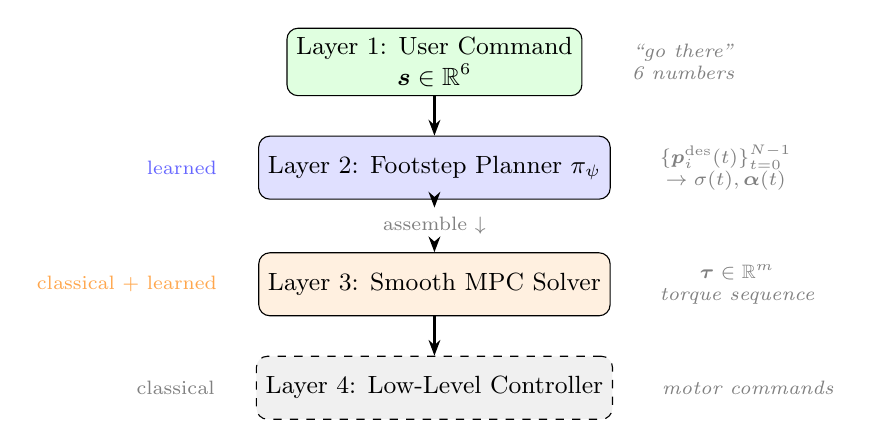
\begin{tikzpicture}[
  block/.style={draw, rounded corners, minimum height=0.8cm,
    minimum width=2.8cm, align=center, font=\small},
  user/.style={block, fill=green!12},
  learned/.style={block, fill=blue!12},
  classical/.style={block, fill=orange!12},
  hw/.style={block, fill=gray!12, dashed},
  arr/.style={-{Stealth[length=2mm]}, thick},
  lbl/.style={font=\scriptsize\itshape, text=gray,
    align=center}
]

% Vertical layout
\node[user] (cmd) {Layer 1: User Command\\$\bm{s} \in \R^6$};
\node[learned, below=0.5cm of cmd] (planner)
  {Layer 2: Footstep Planner $\pi_\psi$};
\node[below=0.1cm of planner, font=\scriptsize, text=gray]
  (mid) {assemble $\downarrow$};
\node[classical, below=0.1cm of mid] (mpc)
  {Layer 3: Smooth MPC Solver};
\node[hw, below=0.5cm of mpc] (hw)
  {Layer 4: Low-Level Controller};

% Side annotations
\node[lbl, right=0.5cm of cmd] {``go there''\\6 numbers};
\node[lbl, right=0.5cm of planner]
  {$\{\bp^{\mathrm{des}}_i(t)\}_{t=0}^{N-1}$\\
   $\to \sigma(t), \balpha(t)$};
\node[lbl, right=0.5cm of mpc]
  {$\bm{\tau} \in \R^m$\\torque sequence};
\node[lbl, right=0.5cm of hw] {motor commands};

% Arrows
\draw[arr] (cmd) -- (planner);
\draw[arr] (planner) -- (mid);
\draw[arr] (mid) -- (mpc);
\draw[arr] (mpc) -- (hw);

% Left side: learned vs classical
\node[font=\scriptsize, left=0.4cm of planner,
  text=blue!60] {learned};
\node[font=\scriptsize, left=0.4cm of mpc,
  text=orange!70] {classical + learned};
\node[font=\scriptsize, left=0.4cm of hw,
  text=gray] {classical};

\end{tikzpicture}
\caption{Four-layer architecture.
  Data flows strictly downward: 6~numbers of intention
  $\to$ $C {\times} 3 {\times} N$ numbers of contact
  geometry $\to$ $m$ torques $\to$ hardware.
  The MPC problem at Layer~3 is \emph{assembled} from the
  reference (Layer~1), contact schedule (Layer~2), dynamics
  (EL-Net), and gains (DARE cache).}
\label{fig:arch}
\end{figure}

\begin{enumerate}
  \item \textbf{User command} $\bm{s} \in \R^6$:
    desired body pose relative to the support polygon.
    This is the only external input.
    Within the MPC horizon, the controller tracks $\bm{s}$
    as a constant reference until the next command arrives.
  \item \textbf{Footstep Planner} (learned, Section~\ref{sec:footstep}):
    maps $(\bx_t, \bm{s}, \cS)$ to a time-stepped sequence
    of desired end-effector positions
    $\bp_i^{\mathrm{des}}(t) \in \R^3$
    for $t = 0, \ldots, N{-}1$.
    The contact mode $\sigma(t)$ and scheduling variable
    $\balpha(t)$ are derived at each timestep
    via~\eqref{eq:sigma}.
  \item \textbf{Smooth MPC solver} (Section~\ref{sec:dare}):
    assembles a time-varying QP from the reference,
    the per-timestep $(\sigma(t), \balpha(t))$,
    the EL-Net dynamics (Section~\ref{sec:elnet}),
    and the DARE-cached gains; then solves it via ADMM.
  \item \textbf{Low-level controller} (classical):
    executes the resulting joint torques on hardware
    via PD tracking or inverse dynamics.
\end{enumerate}

\subsection{Footstep Planner Network}\label{sec:footstep}

\textbf{User command.}
The operator provides a body-pose command
$\bm{s} \in \R^6$, specifying the desired position and
orientation of the center of mass relative to the
support polygon (three translational, three rotational
degrees of freedom).
This is the \emph{only} external specification.
Within the MPC predictive horizon, the controller tracks
$\bm{s}$ as a constant reference until the next command arrives.

\textbf{Time-stepped foot placement sequence.}
The Footstep Planner is a neural network that outputs
a foot-placement sequence over the full MPC horizon:
\begin{equation}\label{eq:planner}
  \pi_\psi : \R^n \times \R^6 \times \cS
  \;\to\; \R^{N \times C \times 3},
\end{equation}
mapping the current state $\bx$, user command $\bm{s}$,
and contact surface $\cS$ to desired end-effector positions
$\bp_i^{\mathrm{des}}(t) \in \R^3$
for each contact point $i = 1, \ldots, C$ and each
timestep $t = 0, \ldots, N{-}1$ of the predictive horizon.

The contact mode at each timestep is derived:
\begin{equation}\label{eq:sigma_derived}
  \sigma_i(t) = \begin{cases}
    1 & \text{if } \phi\bigl(\bp_i^{\mathrm{des}}(t)\bigr) = 0, \\
    0 & \text{if } \phi\bigl(\bp_i^{\mathrm{des}}(t)\bigr) > 0.
  \end{cases}
\end{equation}
This means the Planner outputs a complete \emph{contact schedule
with timing}: it specifies not only which feet are in contact,
but when each contact is made or broken, and where each foot
lands.
The mode sequence $\{\sigma(t)\}_{t=0}^{N-1}$ can vary
within a single MPC horizon---for example, a trot step
may begin with $\sigma = (1,0,1,0)$ and transition to
$(0,1,0,1)$ midway through the horizon.

\textbf{Why positions, not modes.}
This formulation resolves a fundamental issue with directly
predicting $\sigma$: a bare mode classifier cannot express
\emph{where} a foot should land (making contact) or
\emph{how far} it should lift (breaking contact).
By outputting continuous positions, the Planner simultaneously
specifies the contact mode, the contact geometry, and the
swing-leg trajectory.

\textbf{Relationship to WBC gait scheduling.}
In the MIT Cheetah pipeline~\cite{kim2019}, the gait scheduler
is a finite-state machine that cycles through pre-defined
contact modes at fixed timing (e.g., trot: alternating
diagonal pairs at a fixed frequency).
Our Footstep Planner replaces this with a learned policy
that adapts both \emph{timing} and \emph{placement}
to terrain and velocity.
Pre-defined gaits can serve as a \emph{bootstrapping curriculum}:
initialize the Planner to reproduce a trot gait,
then fine-tune via reinforcement learning on varied terrain.

\textbf{Training.}
The Planner is trained via policy gradient methods
(REINFORCE~\cite{williams1992} or PPO~\cite{schulman2017}),
with the tracking cost of the downstream DARE-cached MPC
as the reward signal.
The EL-Net and DARE cache are frozen during Planner training.

\begin{remark}[No Soft Mode Mixing]\label{rem:mixing}
One might consider a differentiable relaxation: replace the
hard mode selection~\eqref{eq:sigma_derived} with soft weights
$w_\sigma$ and blend dynamics as
$A_{\mathrm{eff}} = \sum_\sigma w_\sigma A_\sigma$.
This is \emph{physically meaningless}: a convex combination
of ``foot-on-ground'' and ``foot-in-air'' dynamics
does not correspond to any realizable physical system.
The DARE solution of the blended system does not produce
a useful controller for either mode.
This is fundamentally different from soft attention in
sequence models, where convex combinations of
representations are semantically meaningful.
The discrete mode boundary is precisely where end-to-end
differentiability breaks---and the reason for the two-stage
training architecture.
\end{remark}

\subsection{EL-Net: Euler--Lagrangian Structured Dynamics}
\label{sec:elnet}

Within each contact mode $\sigma$, the dynamics are smooth.
We learn them using a neural network that preserves the
Euler--Lagrange structure of mechanical systems.

\begin{definition}[EL-Net]\label{def:elnet}
For a mechanical system with generalized coordinates
$\bq \in \R^{n_q}$, an \emph{Euler--Lagrangian Network}
(EL-Net) parameterizes:
\begin{enumerate}
  \item \textbf{Inertia matrix}
    $M_\theta(\bq) \in \Spp^{n_q}$
    via Cholesky factorization:
    $M_\theta = L_\theta(\bq) \, L_\theta(\bq)^\top$,
    where $L_\theta$ is a lower-triangular matrix-valued
    neural network with positive diagonal entries.
    This guarantees $M_\theta \succ 0$ by construction.
  \item \textbf{Potential energy}
    $V(\bq) = V_{\mathrm{grav}}(\bq;\, \bm{g},\, \cW)
              + V_\theta(\bq)$,
    where $V_{\mathrm{grav}}(\bq) = -m \, \bm{g}^\top
    \bp_{\mathrm{com}}(\bq)$
    is the known gravitational potential (from $\cW$)
    and $V_\theta(\bq)$ is a scalar-valued neural network
    capturing internal elastic and dissipative potentials.
  \item \textbf{Coriolis matrix}
    $C_\theta(\bq, \dot{\bq})$ derived from $M_\theta$ via
    the Christoffel symbols of the first kind:
    \begin{equation}\label{eq:christoffel}
      [C_\theta]_{ij}
      = \sum_{k=1}^{n_q} \frac{1}{2}
        \Bigl(
          \frac{\partial [M_\theta]_{ij}}{\partial q_k}
          + \frac{\partial [M_\theta]_{ik}}{\partial q_j}
          - \frac{\partial [M_\theta]_{jk}}{\partial q_i}
        \Bigr) \dot{q}_k.
    \end{equation}
    This construction guarantees that
    $\dot{M}_\theta - 2 C_\theta$ is skew-symmetric,
    which is the passivity condition.
\end{enumerate}
\end{definition}

The equations of motion within mode $\sigma$ are:
\begin{equation}\label{eq:eom}
  M_\theta(\bq) \, \ddot{\bq}
  + C_\theta(\bq, \dot{\bq}) \, \dot{\bq}
  + \nabla_{\bq} V(\bq)
  = B_\sigma \, \bu
  + J_\sigma(\bq)^\top \bm{\lambda},
\end{equation}
where $B_\sigma$ is the actuator input matrix
(known from the kinematic chain and mode $\sigma$),
$J_\sigma(\bq)$ is the contact Jacobian for the active
contact points in mode $\sigma$,
and $\bm{\lambda}$ are the contact forces
(eliminated by the holonomic constraints).

\textbf{Guaranteed properties.}
\begin{enumerate}
  \item \emph{SPD inertia}: $M_\theta \succ 0$ by the
    Cholesky parameterization.
  \item \emph{Energy conservation}: the skew-symmetry of
    $\dot{M}_\theta - 2 C_\theta$ is automatic from the
    Christoffel construction~\eqref{eq:christoffel}.
  \item \emph{Passivity}: follows from energy conservation
    and positive-definite dissipation~\cite{lutter2019}.
\end{enumerate}

\textbf{Linearization.}
At an equilibrium $(\bq^*, \dot{\bq}^* = 0)$ within
mode $\sigma$ with scheduling variable $\balpha$,
the linearized dynamics are:
\begin{align}\label{eq:AB_elnet}
  A_\sigma(\balpha)
  &= \begin{pmatrix}
      0 & I \\
      -M_\theta^{-1} H_V & -M_\theta^{-1} C_\theta
    \end{pmatrix}, \notag \\
  B_\sigma(\balpha)
  &= \begin{pmatrix}
      0 \\
      M_\theta^{-1} B_\sigma
    \end{pmatrix},
\end{align}
where $H_V = \nabla^2_{\bq} V(\bq^*)$ is the Hessian of the
potential energy evaluated at the equilibrium,
and all quantities are functions of $\balpha$ through $\bq^*(\balpha)$.

When specialized to the quadrotor with $\sigma = \bm{0}$
(no contacts, no constraints), $J_\sigma = 0$ and
$\bm{\lambda} = 0$, and~\eqref{eq:AB_elnet} reduces to
the block structure of~\cite[Eq.~(5)]{zhang2025flat}
with $G(\balpha)$ playing the role of $-M^{-1} H_V$.

\textbf{Training.}
The EL-Net for each mode $\sigma$ is trained on trajectory data
$\{(\bq_t, \dot{\bq}_t, \bu_t, \ddot{\bq}_t)\}$ collected
from simulation or hardware.
The loss is the prediction error on $\ddot{\bq}$:
\begin{equation}\label{eq:elnet_loss}
  \mathcal{L}_{\mathrm{EL}}(\theta)
  = \sum_t \bigl\|
      \ddot{\bq}_t - M_\theta(\bq_t)^{-1}
      \bigl( B_\sigma \bu_t - C_\theta \dot{\bq}_t
             - \nabla V(\bq_t) \bigr)
    \bigr\|^2.
\end{equation}
The Christoffel matrix $C_\theta$ and the potential gradient
$\nabla V$ are obtained by automatic differentiation through
$M_\theta$ and $V_\theta$, respectively.
Because $V_{\mathrm{grav}}$ is known analytically, the network
$V_\theta$ only needs to learn the internal potential---a
simpler function.

\subsection{DARE Cache and Gain Interpolation}\label{sec:dare}

This component is identical in structure
to~\cite{zhang2025flat}, but applied per mode $\sigma$.

\textbf{Offline.}
For each reachable mode $\sigma \in \cI$ and a grid
$\{\balpha^{(j)}\}_{j=1}^{M_\sigma}$ of scheduling variables:
\begin{enumerate}
  \item Query the EL-Net to obtain
    $A_\sigma(\balpha^{(j)})$, $B_\sigma(\balpha^{(j)})$.
  \item Discretize: $A_d = I + A_\sigma \Delta t$,
    $B_d = B_\sigma \Delta t$.
  \item Solve the augmented DARE~\cite{tinympc}:
    \begin{equation}\label{eq:dare}
      P = Q_\rho + A_d^\top P \bigl(
        A_d - B_d (R_\rho + B_d^\top P B_d)^{-1}
        B_d^\top P A_d \bigr),
    \end{equation}
    where $Q_\rho = Q + \rho I$, $R_\rho = R + \rho I$
    are ADMM-augmented cost matrices.
  \item Compute gain $K_\infty^{(j)}
    = (R_\rho + B_d^\top P B_d)^{-1} B_d^\top P A_d$
    and cache $\{A_d, B_d, K_\infty, P, C_1, C_2\}^{(\sigma, j)}$.
\end{enumerate}

\begin{algorithm}[t]
\caption{Online: Assembled Switched LPV Template MPC}
\label{alg:online}
\begin{algorithmic}[1]
\REQUIRE State $\bx_t$, command $\bm{s}$, surface $\cS$,
  DARE caches
\STATE \textit{--- Layer 2: Footstep Planner ---}
\STATE $\{\bp^{\mathrm{des}}_i(k)\}_{k=0}^{N-1}
  \gets \pi_\psi(\bx_t, \bm{s}, \cS)$
\FOR{$k = 0, \ldots, N{-}1$}
  \STATE $\sigma(k) \gets$ derive
    from $\phi(\bp_i^{\mathrm{des}}(k))$~\eqref{eq:sigma_derived}
  \STATE $\balpha(k) \gets$ extract from
    $(\bx_t, \bp^{\mathrm{des}}(k), \sigma(k))$
    \hfill\textit{Def.~\ref{def:alpha}}
\ENDFOR
\STATE \textit{--- Layer 3: Assemble \& Solve MPC ---}
\FOR{$k = 0, \ldots, N{-}1$}
  \STATE $(A_d, B_d, K_\infty, \ldots)^{(k)} \gets
    \text{CacheLookup}\bigl(\sigma(k), \balpha(k)\bigr)$
  \STATE $(\bx^*, \bu^*)^{(k)} \gets
    \text{Equilibrium}\bigl(\sigma(k), \balpha(k)\bigr)$
\ENDFOR
\STATE $\bx_{\mathrm{ref}} \gets$ from $\bm{s}$
  \hfill\textit{user command $\to$ reference}
\STATE Run $K$ ADMM iterations with time-varying
  $\{A_d, B_d, K_\infty\}^{(k)}$
\STATE $\bu_t \gets \bu^{*(0)} + \delta \bu_0$
\end{algorithmic}
\end{algorithm}

\textbf{MPC problem assembly (Algorithm~\ref{alg:online}).}
The MPC problem is not passed through a monolithic solver.
At each control step, the complete time-varying quadratic program
is \emph{assembled} from four independently sourced components:

\begin{center}
\small
\begin{tabular}{@{}lll@{}}
\toprule
Source & Provides & Role in QP \\
\midrule
User command $\bm{s}$ & $\bx_{\mathrm{ref}}$ & Reference trajectory \\
Footstep Planner & $\sigma(k)$, $\balpha(k)$ & Constraints, scheduling \\
EL-Net$_{\sigma(k)}$ & $A_d(k)$, $B_d(k)$ & Dynamics matrices \\
DARE cache & $K_\infty(k)$, $P(k)$ & Feedback gains \\
\bottomrule
\end{tabular}
\end{center}

\noindent
Because the Planner outputs a time-stepped sequence,
the mode $\sigma(k)$ and scheduling variable $\balpha(k)$
can vary \emph{within} the MPC horizon.
The resulting QP has time-varying dynamics---the matrices
$(A_d, B_d)$ change at each timestep $k$---but each
per-step ADMM pass still uses only cached matrix-vector
products.

\textbf{Zero-iteration variant.}
As in~\cite{zhang2025flat}, the gain can be approximated by
first-order Taylor expansion around a reference
$\balpha_0$ within each mode:
\begin{equation}\label{eq:K_interp}
  K_\sigma(\balpha) \approx K_\sigma(\balpha_0)
  + \sum_{i=1}^{d_\sigma} \delta\alpha_i \;
    \frac{\partial K_\sigma}{\partial \alpha_i},
\end{equation}
where the gain sensitivities $\partial_i K_\sigma$
are computed offline by central differences.
The online cost is then $O(n \cdot m \cdot d_\sigma)$
multiply-accumulate operations.

\subsection{Training Pipeline}\label{sec:training}

The three learned components---EL-Nets, DARE caches, and
Footstep Planner---are trained in a three-stage pipeline
(Algorithm~\ref{alg:offline}).
The stages are sequential: the DARE cache requires
trained EL-Nets, and the Planner reward requires a
functional DARE-cached controller.
An optional fourth stage performs within-mode joint
fine-tuning via implicit DARE differentiation.

\textbf{Stage~1: EL-Net (supervised, per mode).}
For each mode $\sigma$, trajectory data
$\mathcal{D}_\sigma = \{(\bq_t, \dot{\bq}_t,
\bu_t, \ddot{\bq}_t)\}$ is collected from a MuJoCo
simulator~\cite{todorov2012} operating in mode $\sigma$.
The EL-Net parameters $\theta_\sigma$ are updated by
gradient descent on~\eqref{eq:elnet_loss}.
The gradient flows through the Christoffel
construction~\eqref{eq:christoffel} and the potential
$V_\theta$ via automatic differentiation.
The \emph{Push--Prove--Pull} structure is:
\begin{align}
  \text{Push:}\; &\theta \to (M_\theta, V_\theta, C_\theta)
    \to \hat{\ddot{\bq}}, \notag\\
  \text{Prove:}\; &\mathcal{L}_{\mathrm{EL}}
    = \|\ddot{\bq} - \hat{\ddot{\bq}}\|^2,
    \label{eq:ppp_elnet}\\
  \text{Pull:}\; &\theta \gets \theta
    - \eta \, \nabla_\theta \mathcal{L}_{\mathrm{EL}}.
    \notag
\end{align}

\textbf{Stage~2: DARE cache (numerical).}
Using the trained EL-Nets, the DARE cache is built
for each mode $\sigma$ over a grid of scheduling variables
as described in Section~\ref{sec:dare}.
No learning; pure numerical linear algebra.

\textbf{Stage~3: Footstep Planner (RL).}
With EL-Nets and DARE caches frozen, the Planner $\pi_\psi$
is trained by sampling $N$ foot-placement sequences,
rolling them forward through the DARE-cached MPC in MuJoCo,
and reweighting by trajectory cost via Boltzmann
weights~\cite{williams2017}:
\begin{equation}\label{eq:boltzmann}
  w^{(n)} = \frac{\exp\bigl(-L^{(n)} / \lambda\bigr)}
    {\sum_{n'} \exp\bigl(-L^{(n')} / \lambda\bigr)},
\end{equation}
where $L^{(n)} = \sum_{t}
\bigl(\|\bx_t - \bx_{\mathrm{ref}}\|_Q^2
      + \|\bu_t\|_R^2\bigr)$
is the tracking cost of rollout $n$
and $\lambda > 0$ is a temperature.
The Planner parameters are updated via:
\begin{equation}\label{eq:planner_grad}
  \psi \gets \psi - \eta_\psi \sum_{n=1}^N
    w^{(n)} \nabla_\psi \log
    \pi_\psi(\bp^{(n)} \mid \bx, \bm{s}).
\end{equation}
Pre-defined gaits (trot, walk, gallop) initialize
$\pi_\psi$ via behavioral cloning before RL fine-tuning.

\textbf{Stage~4 (optional): Within-mode fine-tuning.}
Within a fixed mode $\sigma$, the full chain
from EL-Net through DARE to tracking cost
is differentiable:
\begin{align}
  \text{Push:}\; &\theta \to
    (A_\sigma(\balpha), B_\sigma(\balpha)),
    \notag\\
  \text{Prove:}\; &\text{DARE}
    \to K_\infty \to \bu \to
    \mathcal{L}_{\mathrm{track}},
    \label{eq:ppp_finetune}\\
  \text{Pull:}\; &\theta \gets \theta
    - \eta \, \partial \mathcal{L}_{\mathrm{track}}
    / \partial\theta
    \;\;\text{(Lyap.~\eqref{eq:lyap})}.
    \notag
\end{align}
This fine-tunes EL-Net weights to minimize downstream
MPC tracking error, not just acceleration prediction error.
The DARE cache is rebuilt after each parameter update.

\begin{algorithm}[t]
\caption{Offline Training (MuJoCo Simulator)}
\label{alg:offline}
\begin{algorithmic}[1]
\REQUIRE Simulator $f_{\mathrm{sim}}$, modes $\cI$,
  $\balpha$-grids, $Q, R, \rho$
\STATE \textit{--- Stage 1: EL-Net (per mode) ---}
\FOR{each $\sigma \in \cI$}
  \STATE $\mathcal{D}_\sigma \gets$ collect
    $(\bq, \dot{\bq}, \bu, \ddot{\bq})$
    from $f_{\mathrm{sim}}$ in mode $\sigma$
  \FOR{epoch $= 1, \ldots, E_1$}
    \STATE $\theta_\sigma \gets \theta_\sigma
      - \eta_1 \nabla_{\theta_\sigma}
      \mathcal{L}_{\mathrm{EL}}$
      \hfill\eqref{eq:elnet_loss}
  \ENDFOR
\ENDFOR
\STATE \textit{--- Stage 2: DARE cache ---}
\FOR{each $\sigma \in \cI$, grid point $\balpha^{(j)}$}
  \STATE $(A_d, B_d) \gets$ discretize
    EL-Net$_\sigma(\balpha^{(j)})$
  \STATE DARE~\eqref{eq:dare}
    $\to (K_\infty, P)^{(\sigma, j)}$
  \STATE $\partial_i K_\sigma \gets$ central differences
\ENDFOR
\STATE \textit{--- Stage 3: Footstep Planner (RL) ---}
\STATE Init $\pi_\psi \gets$
  behavioral clone of pre-defined gait
\FOR{iter $= 1, \ldots, I_3$}
  \FOR{$n = 1, \ldots, N$}
    \STATE $\{\bp_i^{(n)}\} \gets
      \pi_\psi(\bx, \bm{s}, \cS) + \epsilon_n$
    \STATE Roll out in $f_{\mathrm{sim}}$
      with Alg.~\ref{alg:online}
    \STATE $L^{(n)} \gets$ trajectory cost
  \ENDFOR
  \STATE $w^{(n)} \gets$ Boltzmann~\eqref{eq:boltzmann}
  \STATE $\psi \gets \psi
    - \eta_\psi \sum_n w^{(n)}
      \nabla_\psi \log \pi_\psi$
    \hfill\eqref{eq:planner_grad}
\ENDFOR
\STATE \textit{--- Stage 4 (opt): Fine-tune per mode ---}
\FOR{each $\sigma$, epoch $= 1, \ldots, E_4$}
  \STATE $\nabla_\theta \mathcal{L}_{\mathrm{track}}
    \gets$ \eqref{eq:grad_chain} via Lyap.~\eqref{eq:lyap}
  \STATE $\theta_\sigma \gets \theta_\sigma
    - \eta_4 \nabla_\theta \mathcal{L}_{\mathrm{track}}$;
    rebuild cache
\ENDFOR
\RETURN $\{\theta_\sigma\}, \text{caches}, \psi$
\end{algorithmic}
\end{algorithm}

\begin{algorithm}[t]
\caption{Online Deployment (Real Robot)}
\label{alg:deploy}
\begin{algorithmic}[1]
\REQUIRE Trained $\pi_\psi$, EL-Nets $\{\theta_\sigma\}$,
  DARE caches, sensors
\STATE Load caches and weights to onboard memory
\STATE $\mathcal{D}_{\mathrm{on}} \gets \emptyset$
  \hfill (adaptation buffer)
\LOOP
  \STATE $\bm{s} \gets$ user body-pose command
    \hfill (6 numbers)
  \STATE $\bx_t \gets$ IMU + joint encoders
  \STATE $\cS \gets$ depth camera
    \hfill (terrain SDF)
  \STATE \textit{--- Layer 2: Plan ---}
  \STATE $\{\bp_i^{\mathrm{des}}(k)\}_{k=0}^{N-1}
    \gets \pi_\psi(\bx_t, \bm{s}, \cS)$
  \FOR{$k = 0, \ldots, N{-}1$}
    \STATE $\sigma(k), \balpha(k) \gets$
      derive from $\phi(\bp_i^{\mathrm{des}}(k))$
  \ENDFOR
  \STATE \textit{--- Layer 3: Assemble \& Solve
    (Alg.~\ref{alg:online}) ---}
  \STATE $\bu_t \gets$ DARE-cached ADMM
    with time-varying $\{\sigma(k), \balpha(k)\}$
  \STATE \textit{--- Layer 4: Execute ---}
  \STATE Apply $\bu_t$ to motors
  \STATE \textit{--- Online Adaptation (periodic) ---}
  \STATE $\mathcal{D}_{\mathrm{on}} \gets
    \mathcal{D}_{\mathrm{on}} \cup
    \{(\bq_t, \dot{\bq}_t, \bu_t, \ddot{\bq}_t)\}$
  \IF{$|\mathcal{D}_{\mathrm{on}}|
      \geq B_{\mathrm{adapt}}$}
    \STATE $\theta_{\sigma_t} \gets \theta_{\sigma_t}
      - \eta_{\mathrm{a}} \nabla_\theta
      \mathcal{L}_{\mathrm{EL}}
        (\mathcal{D}_{\mathrm{on}})$
    \STATE Rebuild cache for current $(\sigma, \balpha)$
    \STATE $\mathcal{D}_{\mathrm{on}} \gets \emptyset$
  \ENDIF
\ENDLOOP
\end{algorithmic}
\end{algorithm}

\textbf{Why not end-to-end?}
The mode derivation~\eqref{eq:sigma_derived} involves a
hard threshold ($\phi = 0$), blocking gradient flow from
the DARE cache to the Planner.
Remark~\ref{rem:mixing} explains why softening this threshold
is not a valid alternative.
Within each mode, however, the pipeline from EL-Net through
DARE to tracking cost \emph{is} differentiable
(Stage~4), enabling joint fine-tuning
of the EL-Net and cost matrices $Q, R$.

% ================================================================
\section{Analysis}\label{sec:analysis}

\subsection{Generalized Equivalence Chain}

\begin{theorem}[Equivalence Chain]\label{thm:chain}
For a switched LPV system, the following controllers form a
hierarchy of decreasing online computation, with each step
introducing a bounded approximation:
\begin{multline}\label{eq:chain}
  \text{\emph{Full TO}}
  \xrightarrow{\text{fix } \sigma}
  \text{\emph{Mode-Given TO}}
  \xrightarrow{\text{cache DARE}}  \\
  \text{\emph{Template MPC}}
  \xrightarrow{K \to 0}
  \text{\emph{Analytic Template}}
  \xrightarrow{\text{1st ord.}}
  \text{\emph{Gain Sched.}}
\end{multline}
\end{theorem}

\begin{proof}
We trace each arrow.

(i) \emph{Full TO $\to$ Mode-Given TO.}
Full trajectory optimization over both $\sigma$
and $\bu$ (e.g., contact-implicit~\cite{posa2014})
jointly selects the mode sequence and control.
Fixing $\sigma$ via the Footstep Planner yields a
smooth optimal control problem within the selected mode.
The approximation error is bounded by the Planner's
sub-optimality in mode selection.

(ii) \emph{Mode-Given TO $\to$ Template MPC.}
Within mode $\sigma$, online relinearization at each
timestep followed by DARE solve gives the optimal
LQR gain $K_\sigma(\balpha_t)$.
Replacing this with a cached DARE at the nearest
grid point $\balpha^{(j)}$ introduces an error
$\|K_\sigma(\balpha_t) - K_\sigma(\balpha^{(j)})\|$,
bounded by Proposition~\ref{prop:interp_error}
and controlled by grid density.

(iii) \emph{Template MPC $\to$ Analytic Template.}
Setting the number of ADMM iterations $K = 0$
(with zero warm-start) yields
$\bu_0 = \bu^* - K_\infty(\balpha) \, \delta\bx$,
which is the unconstrained LQR feedback.
The error relative to converged ADMM is the
constraint violation~\cite{zhang2025flat}.

(iv) \emph{Analytic Template $\to$ Gain Schedule.}
Replacing $K_\infty(\balpha)$ by the first-order
interpolation~\eqref{eq:K_interp} introduces the
Taylor remainder error (Proposition~\ref{prop:interp_error}).
\end{proof}

\begin{table}[t]
\centering
\caption{Online computational complexity of each controller variant.
  $n$: state dimension, $m$: input dimension, $K$: ADMM iterations,
  $n_\pi$: Planner network size, $d$: scheduling dimension.}
\label{tab:complexity}
\begin{tabular}{@{}lcc@{}}
\toprule
Variant & Online cost & Constraints \\
\midrule
Full TO         & $O(n^3 N)$     & Yes \\
Mode-Given TO   & $O(n^3) + K \cdot O(n^2)$ & Yes \\
Template MPC    & $n_\pi + K \cdot O(n^2)$ & Yes \\
Analytic Templ. & $n_\pi + O(n \cdot m \cdot d)$ & Clip only \\
\bottomrule
\end{tabular}
\end{table}

\subsection{Sufficient Conditions}

\begin{proposition}[Applicability Conditions]
\label{prop:conditions}
The switched LPV Template MPC framework is applicable when:
\begin{enumerate}
  \item \textbf{Finite modes}: The system has a finite number
    of reachable contact modes $|\cI| < \infty$.
  \item \textbf{Intra-mode smoothness}: Within each mode $\sigma$,
    the dynamics $A_\sigma(\balpha)$, $B_\sigma(\balpha)$
    are $\mathcal{C}^2$ functions of $\balpha$.
  \item \textbf{Low-dimensional scheduling}:
    $d_\sigma \ll n$ for all $\sigma \in \cI$.
  \item \textbf{Stabilizability}: For each $(\sigma, \balpha)$,
    the pair $(A_\sigma(\balpha), B_\sigma(\balpha))$
    is stabilizable, so the DARE has a unique
    stabilizing solution.
  \item \textbf{Gain smoothness}: $K_\sigma(\balpha)$
    is $\mathcal{C}^1$ in $\balpha$ with bounded gradient,
    so first-order interpolation has controlled error.
\end{enumerate}
\end{proposition}

Condition (1) excludes continuous contact surfaces
(e.g., rolling) without discretization.
Condition (3) is what makes caching feasible:
a grid over $\R^d$ with $d = 6$ is practical;
a grid over $\R^{36}$ (full quadruped state) is not.
Condition (4) is inherited from standard LQR theory.
Condition (5) follows from condition (2) by the implicit
function theorem applied to the DARE.

\subsection{Gain Interpolation Error}\label{sec:interp}

\begin{proposition}[Interpolation Error Bound]
\label{prop:interp_error}
Let $K_\sigma : \R^{d_\sigma} \to \R^{m \times n}$ be
the DARE gain map for mode $\sigma$, assumed $\mathcal{C}^2$.
Then the first-order interpolation error satisfies
\begin{equation}\label{eq:taylor_bound}
  \bigl\| K_\sigma(\balpha) - K_\sigma(\balpha_0)
    - \nabla_{\!\balpha} K_\sigma(\balpha_0)^\top
      (\balpha - \balpha_0)
  \bigr\|_F
  \leq \frac{\beta_\sigma}{2}
    \|\balpha - \balpha_0\|^2,
\end{equation}
where $\beta_\sigma = \sup_{\balpha}
\|\nabla^2_{\!\balpha} K_\sigma(\balpha)\|$ is the
maximum Hessian norm over the scheduling domain.
\end{proposition}

\begin{proof}
This is the standard multivariate Taylor remainder theorem
applied to the matrix-valued function $K_\sigma$.
The $\mathcal{C}^2$ regularity is guaranteed by
Proposition~\ref{prop:conditions}(2,5).
\end{proof}

For the quadrotor ($d=4$), \cite{zhang2025flat} measured
a mean relative error of 4\% over the tested range.
For a quadruped in trot ($d=6$), we expect comparable accuracy
for moderate COM excursions, with the error growing quadratically
for large deviations from the reference $\balpha_0$.

\subsection{DARE Differentiability}\label{sec:dare_diff}

\begin{proposition}[Implicit Differentiation of DARE]
\label{prop:dare_diff}
The DARE solution $P$ as a function of $(A, B, Q, R)$
is differentiable wherever it exists and is unique.
The gradient $\partial P / \partial A$ is the solution of
a discrete Lyapunov equation:
\begin{equation}\label{eq:lyap}
  \frac{\partial P}{\partial A}
  = A_{\mathrm{cl}}^\top \, \frac{\partial P}{\partial A}
    \, A_{\mathrm{cl}} + F,
\end{equation}
where $A_{\mathrm{cl}} = A - B K_\infty$ is the closed-loop
matrix and $F$ is a forcing term depending on $P$, $K_\infty$,
and the perturbation direction.
\end{proposition}

This enables backpropagation from the MPC tracking cost
through the DARE cache to the EL-Net parameters $\theta$---within
each mode.
The gradient flow is:
\[
  \frac{\partial \mathcal{L}}{\partial \theta}
  = \frac{\partial \mathcal{L}}{\partial K}
    \frac{\partial K}{\partial P}
    \frac{\partial P}{\partial (A,B)}
    \frac{\partial (A,B)}{\partial \theta}.
\]
The chain terminates at the EL-Net; it does not cross
mode boundaries (which require RL, as discussed in
Section~\ref{sec:footstep}).

% ================================================================
\section{Instantiation Examples}\label{sec:examples}

\subsection{Quadrotor: Recovering Paper 1}

The quadrotor has $C = 0$ contact points, so
$\cI = \{\bm{0}\}$ (single mode) and $\cS = \emptyset$.
The scheduling variable is $\balpha = (a_x, a_y, a_z, \psi)$
from differential flatness~\cite{zhang2025flat},
not from the general formula $d_\sigma = 2|\sigma| + 2 = 2$.

The EL-Net is replaced by the analytic flat linearization:
$A(\balpha)$, $B(\balpha)$ are closed-form trigonometric
expressions~\cite[Eq.~(5)]{zhang2025flat}.
The DARE cache is built over a 4D grid of $\balpha$ values.
The Footstep Planner is absent (no contacts to schedule).

The full equivalence chain~\eqref{eq:chain} reduces to the
quadrotor-specific chain of~\cite{zhang2025flat}:
\begin{multline*}
  \text{Online Relin}
  \xrightarrow{\text{cache}}
  \text{Flat Template}
  \xrightarrow{K\to 0}  \\
  \text{Analytic Template}
  \xrightarrow{\text{1st ord.}}
  \text{Gain Sched.}
\end{multline*}
Table~\ref{tab:quad_results} reproduces the key results
from~\cite{zhang2025flat} as validation.

\begin{table}[t]
\centering
\caption{Quadrotor figure-eight tracking~\cite{zhang2025flat}:
  the general framework recovers Paper~1 results.}
\label{tab:quad_results}
\begin{tabular}{@{}lccc@{}}
\toprule
Variant & Avg.\ error (m) & ADMM iters & Speedup \\
\midrule
Online Relin     & 0.035 & 1023 & $1\times$ \\
Flat Template    & 0.035 & 714  & $29\times$ \\
Analytic Templ.  & 0.036 & 0    & $85\times$ \\
\bottomrule
\end{tabular}
\end{table}

\subsection{Quadruped Trot: Worked Example}\label{sec:quad_trot}

Consider a quadruped with $C = 4$ feet.
A trotting gait cycles through contact modes
corresponding to alternating diagonal pairs:

\begin{center}
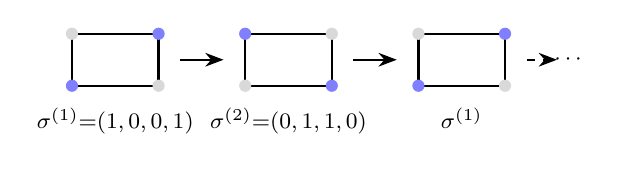
\begin{tikzpicture}[scale=0.55, font=\footnotesize]
  % Phase 1: FL+HR
  \begin{scope}[shift={(0,0)}]
    \draw[thick] (0,0) rectangle (2,1.2);
    \fill[blue!50] (0,0) circle (4pt);     % FL
    \fill[gray!30] (2,0) circle (4pt);     % FR
    \fill[gray!30] (0,1.2) circle (4pt);   % HL
    \fill[blue!50] (2,1.2) circle (4pt);   % HR
    \node[below] at (1,-0.3) {$\sigma^{(1)}{=}(1,0,0,1)$};
  \end{scope}
  % Arrow
  \draw[-{Stealth}, thick] (2.5,0.6) -- (3.5,0.6);
  % Phase 2: FR+HL
  \begin{scope}[shift={(4,0)}]
    \draw[thick] (0,0) rectangle (2,1.2);
    \fill[gray!30] (0,0) circle (4pt);
    \fill[blue!50] (2,0) circle (4pt);
    \fill[blue!50] (0,1.2) circle (4pt);
    \fill[gray!30] (2,1.2) circle (4pt);
    \node[below] at (1,-0.3) {$\sigma^{(2)}{=}(0,1,1,0)$};
  \end{scope}
  % Arrow
  \draw[-{Stealth}, thick] (6.5,0.6) -- (7.5,0.6);
  % Phase 3 = Phase 1
  \begin{scope}[shift={(8,0)}]
    \draw[thick] (0,0) rectangle (2,1.2);
    \fill[blue!50] (0,0) circle (4pt);
    \fill[gray!30] (2,0) circle (4pt);
    \fill[gray!30] (0,1.2) circle (4pt);
    \fill[blue!50] (2,1.2) circle (4pt);
    \node[below] at (1,-0.3) {$\sigma^{(1)}$};
  \end{scope}
  \draw[-{Stealth}, thick, dashed] (10.5,0.6) -- (11.2,0.6);
  \node at (11.5,0.6) {$\cdots$};
\end{tikzpicture}
\end{center}

In each phase, $|\sigma| = 2$ (two feet on ground), so
$d_\sigma = 2 \cdot 2 + 2 = 6$.
The scheduling variable is:
\begin{equation}\label{eq:alpha_trot}
  \balpha_\sigma = \bigl(
    \underbrace{(p_i - p_{\mathrm{com}})_{xy}}_{\text{foot 1}},\;
    \underbrace{(p_j - p_{\mathrm{com}})_{xy}}_{\text{foot 2}},\;
    \underbrace{s_{xy}}_{\text{COM skew}}
  \bigr) \in \R^6,
\end{equation}
where $i, j$ are the indices of the active feet
and $s_{xy}$ is the COM position relative to the midpoint
of the two active feet, projected onto the ground plane.

\textbf{Storage budget.}
For the zero-iteration variant, each mode requires
$K_\sigma(\balpha_0) \in \R^{m \times n}$
plus $d_\sigma$ sensitivity matrices
$\partial_i K_\sigma \in \R^{m \times n}$.
With $m = 12$ (joint torques), $n = 24$ (generalized
coordinates + velocities), $d_\sigma = 6$:
\[
  (1 + 6) \times 12 \times 24 = 2016 \;\text{floats per mode}.
\]
For a trot gait with 2 distinct modes:
$2 \times 2016 = 4032$ floats $\approx$ 16\,kB
(single precision).

\textbf{Comparison with WBC.}
The standard WBC pipeline for this system would use:
(i) a gait scheduler that prescribes $\sigma^{(1)} \to
\sigma^{(2)} \to \sigma^{(1)} \to \cdots$ at fixed timing;
(ii) a rigid-body dynamics model for the contact-consistent
dynamics; and (iii) a QP solver (e.g., qpOASES) to compute
torques online.
Our framework replaces (i) with the Footstep Planner
(adaptive timing and placement),
(ii) with EL-Nets (learned, structured),
and (iii) with DARE-cached feedback (offline solve).
The pre-defined trot gait can initialize the Planner
training.

% ================================================================
\section{Discussion}\label{sec:discussion}

\textbf{Exploration vs.\ exploitation.}
The architecture separates two fundamentally different
computational problems:
\begin{itemize}
  \item \emph{Exploration} (Footstep Planner):
    Which contact sequence leads to a good trajectory?
    This is combinatorial ($2^C$ modes per step) and requires
    search or learning.
    The Planner amortizes this search into a single
    forward pass---analogous to AlphaGo's policy network,
    which replaces game-tree search with pattern
    matching~\cite{silver2016}.
  \item \emph{Exploitation} (EL-Net + DARE cache):
    Given the contact sequence, what is the optimal feedback?
    This is continuous, smooth, and amenable to classical
    control theory.
    The DARE cache enables constant-time lookup---analogous
    to AlphaGo's value network, which replaces rollout
    evaluation with fast inference.
\end{itemize}

\textbf{Limitations.}
\begin{enumerate}
  \item \emph{Mode scaling}: $|\cI| \leq 2^C$
    grows exponentially with the number of contact points.
    For dexterous manipulation ($C \geq 10$), mode clustering
    or hierarchical decomposition is needed.
  \item \emph{Two-stage training}: The Planner and EL-Nets
    cannot be trained end-to-end (Remark~\ref{rem:mixing}).
    This increases engineering complexity compared to
    monolithic RL policies.
  \item \emph{Mode transition dynamics}: The current formulation
    assumes instantaneous mode switching.
    Impact dynamics and guard conditions at mode boundaries
    are not modeled.
  \item \emph{Gain interpolation accuracy}: The first-order
    Taylor approximation~\eqref{eq:K_interp} degrades for
    large $\|\balpha - \balpha_0\|$.
    For $d_\sigma = 6$ (quadruped trot), a second-order
    expansion or denser grid may be needed.
\end{enumerate}

\textbf{Minimal specification.}
In the standard WBC pipeline, the engineer must provide
two objects in addition to the user command:
a gait table (specifying which feet contact the ground and when)
and a dynamics model (specifying inertial parameters, joint
friction, and contact geometry).
Both require expert knowledge and careful tuning.
In our framework, neither is required.
The Footstep Planner learns the contact schedule from
experience; the EL-Net learns the dynamics from data.
The only human input is $\bm{s} \in \R^6$: six numbers
specifying where the body should be.
Everything else is either learned or derived from
classical control theory.
This is the sharpest possible form of the WBC decomposition:
retain the layered structure (which is architecturally sound)
while eliminating all pre-specified domain knowledge.

\textbf{What is classical vs.\ what is new.}
Gain scheduling~\cite{rugh2000}, LPV control~\cite{shamma1991},
Euler--Lagrangian learning~\cite{lutter2019},
and Riccati sensitivity~\cite{hewer1971,konstantinov1993}
are individually well established.
Our contribution is their integration into a modular
four-layer architecture for contact-rich MPC:
(i)~the state decomposition (COM skew + relative foot positions)
that yields an exactly determined, low-dimensional scheduling
variable;
(ii)~the time-stepped Footstep Planner that outputs a complete
contact schedule with geometry over the MPC horizon;
(iii)~the assembled MPC formulation where each component of
the QP is sourced independently;
(iv)~the identification of Remark~\ref{rem:mixing}---that
soft mode mixing is physically meaningless---as the
fundamental reason for two-stage training.

% ================================================================
\section{Conclusion}\label{sec:conclusion}

We presented a four-layer architecture for real-time MPC
of contact-rich robotic systems in which the only external
specification is a six-dimensional body-pose command.
The Footstep Planner (Layer~2) outputs a time-stepped
contact schedule over the MPC horizon;
the EL-Nets provide structured per-mode dynamics;
the DARE cache enables constant-time feedback.
The MPC problem at each timestep is assembled from these
independently sourced components, not solved monolithically.

The quadrotor result of~\cite{zhang2025flat} is recovered
as a single-mode special case with analytic dynamics.
For quadruped trotting, the scheduling variable has
dimension $d = 6$, yielding a storage budget of
${\sim}16$\,kB and practical computation requirements.

Future work includes:
hardware deployment on the Unitree Go2 platform,
extension to dexterous manipulation via mode clustering,
online adaptation of EL-Net weights via meta-learning,
and formal switched-system stability analysis
with dwell-time constraints.

\medskip
\noindent\textit{Yes, this is what you need to train a robot:
a completed Yang--Mills theory.
And this is what was missing.}

% ================================================================
% APPENDICES
% ================================================================
\appendix

\section{EL-Net Linearization Derivation}\label{app:linearization}

We derive the linearized dynamics~\eqref{eq:AB_elnet}
from the EL equations of motion~\eqref{eq:eom}.

Consider an equilibrium $(\bq^*, \dot{\bq}^* = 0, \bu^*)$
within mode $\sigma$.
Define perturbations $\delta\bq = \bq - \bq^*$,
$\delta\dot{\bq} = \dot{\bq}$,
$\delta\bu = \bu - \bu^*$.

The EL equations at the equilibrium satisfy:
\begin{equation}\label{eq:eom_eq}
  \nabla_{\bq} V(\bq^*) = B_\sigma \bu^*
    + J_\sigma(\bq^*)^\top \bm{\lambda}^*.
\end{equation}

Linearizing~\eqref{eq:eom} about this equilibrium
and subtracting~\eqref{eq:eom_eq}:
\begin{equation}\label{eq:eom_lin}
  M^* \, \delta\ddot{\bq}
  + C^* \, \delta\dot{\bq}
  + H_V \, \delta\bq
  = B_\sigma \, \delta\bu
  + \underbrace{
    \frac{\partial}{\partial \bq}
    \bigl(J_\sigma^\top \bm{\lambda}\bigr)
    \Big|_{*}}_{\text{contact stiffness}} \delta\bq,
\end{equation}
where $M^* = M_\theta(\bq^*)$,
$C^* = C_\theta(\bq^*, 0)$ (which vanishes at
$\dot{\bq}^* = 0$ by the Christoffel
construction~\eqref{eq:christoffel}),
and $H_V = \nabla^2_{\bq} V(\bq^*)$.

For rigid contacts (infinite stiffness), the contact
term is absorbed into the holonomic constraint
$J_\sigma \, \delta\bq = 0$, and the linearization
reduces to the constrained form.
In the unconstrained generalized coordinates
(after projecting out the constrained directions),
we obtain the state-space form:
\[
  \frac{d}{dt}
  \begin{pmatrix} \delta\bq \\ \delta\dot{\bq} \end{pmatrix}
  =
  \underbrace{
  \begin{pmatrix}
    0 & I \\
    -(M^*)^{-1} H_V & 0
  \end{pmatrix}
  }_{A_\sigma(\balpha)}
  \begin{pmatrix} \delta\bq \\ \delta\dot{\bq} \end{pmatrix}
  +
  \underbrace{
  \begin{pmatrix}
    0 \\
    (M^*)^{-1} B_\sigma
  \end{pmatrix}
  }_{B_\sigma(\balpha)}
  \delta\bu,
\]
which is~\eqref{eq:AB_elnet} with $C^* = 0$ at the equilibrium.

When specialized to the quadrotor:
$M^* = m I_3$ (scalar mass, no rotational coupling in
translational dynamics),
$H_V = -m \, \partial^2 V_{\mathrm{grav}}/\partial \bq^2
       = G(\balpha)$ (the gravity coupling matrix
of~\cite[Eq.~(5)]{zhang2025flat}),
and $B_\sigma = k_t \cdot [\text{thrust direction}]$,
recovering the quadrotor-specific block structure.

\section{DARE Implicit Differentiation}\label{app:dare_diff}

The DARE~\eqref{eq:dare} defines $P$ implicitly as a function
of $(A, B, Q, R)$.
Define the residual:
\begin{equation}\label{eq:dare_residual}
  F(P, A, B) \triangleq P - Q_\rho
    - A^\top P (A - B K(P)) = 0,
\end{equation}
where $K(P) = (R_\rho + B^\top P B)^{-1} B^\top P A$.

By the implicit function theorem,
$\partial P / \partial A$ satisfies:
\[
  \frac{\partial F}{\partial P} \cdot
  \frac{\partial P}{\partial A}
  = - \frac{\partial F}{\partial A}.
\]

The operator $\partial F / \partial P$ acts on a perturbation
$\Delta P$ as:
\[
  \frac{\partial F}{\partial P}[\Delta P]
  = \Delta P - A_{\mathrm{cl}}^\top \, \Delta P \, A_{\mathrm{cl}},
\]
where $A_{\mathrm{cl}} = A - B K$ is the closed-loop matrix
(stable by the DARE solution).

Therefore, $\partial P / \partial A$ is the solution of the
\emph{discrete Lyapunov equation}:
\begin{equation}\label{eq:lyap_full}
  \Delta P - A_{\mathrm{cl}}^\top \, \Delta P \, A_{\mathrm{cl}}
  = \frac{\partial F}{\partial A},
\end{equation}
which has a unique solution because $A_{\mathrm{cl}}$ is stable
(all eigenvalues inside the unit circle).
This is solvable in $O(n^3)$ by the Bartels--Stewart
algorithm~\cite{bartels1972}.

The complete gradient chain for EL-Net training is:
\begin{align}
  \frac{\partial \mathcal{L}}{\partial \theta}
  &= \frac{\partial \mathcal{L}}{\partial \bu}
     \frac{\partial \bu}{\partial K}
     \frac{\partial K}{\partial P}
     \frac{\partial P}{\partial (A_d, B_d)}
     \frac{\partial (A_d, B_d)}{\partial (A_c, B_c)}
     \frac{\partial (A_c, B_c)}{\partial \theta},
     \label{eq:grad_chain}
\end{align}
where $\partial(A_d, B_d)/\partial(A_c, B_c)$ is the
discretization Jacobian ($\Delta t \cdot I$ for forward Euler),
and $\partial(A_c, B_c)/\partial\theta$ is obtained by
automatic differentiation through the EL-Net.

This gradient chain enables fine-tuning EL-Net weights
to minimize downstream tracking cost, \emph{within} a fixed
contact mode.
It does \emph{not} cross mode boundaries---those require
the RL-based Footstep Planner training of
Section~\ref{sec:footstep}.

% ================================================================
\bibliographystyle{IEEEtran}
\begin{thebibliography}{20}

\bibitem{zhang2025flat}
J.~Zhang,
``TinyMPC with differential flatness:
$\alpha$-parameterized templates for efficient quadrotor control,''
2025, preprint.

\bibitem{tinympc}
A.~Alavilli, K.~Nguyen, S.~Schoedel, B.~Plancher, and Z.~Manchester,
``TinyMPC: Model-predictive control on resource-constrained
microcontrollers,''
in \emph{Proc.\ IEEE ICRA}, 2024.

\bibitem{kim2019}
S.~Kim, D.~Kim, and S.~Kim,
``Highly dynamic quadruped locomotion via whole-body impulse control
and model predictive control,''
2019, arXiv:1909.06586.

\bibitem{posa2014}
M.~Posa, C.~Cantu, and R.~Tedrake,
``A direct method for trajectory optimization of rigid bodies
through contact,''
\emph{Int.\ J.\ Robotics Research}, vol.~33, no.~1,
pp.~69--81, 2014.

\bibitem{lutter2019}
M.~Lutter, C.~Ritter, and J.~Peters,
``Deep Lagrangian Networks: Using physics as model prior for
deep learning,''
in \emph{Proc.\ ICLR}, 2019.

\bibitem{mellinger2011}
D.~Mellinger and V.~Kumar,
``Minimum snap trajectory generation and control for quadrotors,''
in \emph{Proc.\ IEEE ICRA}, 2011, pp.~2520--2525.

\bibitem{murray1995}
R.~M.~Murray, M.~Rathinam, and W.~Sluis,
``Differential flatness of mechanical control systems,''
in \emph{Proc.\ ASME IMECE}, 1995.

\bibitem{rugh2000}
W.~J.~Rugh and J.~S.~Shamma,
``Research on gain scheduling,''
\emph{Automatica}, vol.~36, no.~10, pp.~1401--1425, 2000.

\bibitem{shamma1991}
J.~S.~Shamma and M.~Athans,
``Guaranteed properties of gain scheduled control for linear
parameter-varying plants,''
\emph{Automatica}, vol.~27, no.~3, pp.~559--564, 1991.

\bibitem{hewer1971}
G.~A.~Hewer,
``An iterative technique for the computation of the steady state
gains for the discrete optimal regulator,''
\emph{IEEE Trans.\ Automatic Control}, vol.~16, no.~4,
pp.~382--384, 1971.

\bibitem{konstantinov1993}
M.~M.~Konstantinov, P.~Hr.~Petkov, and N.~D.~Christov,
``Perturbation analysis of the discrete Riccati equation,''
\emph{Kybernetika}, vol.~29, no.~1, pp.~18--29, 1993.

\bibitem{williams1992}
R.~J.~Williams,
``Simple statistical gradient-following algorithms for
connectionist reinforcement learning,''
\emph{Machine Learning}, vol.~8, pp.~229--256, 1992.

\bibitem{schulman2017}
J.~Schulman, F.~Wolski, P.~Dhariwal, A.~Radford, and O.~Klimov,
``Proximal policy optimization algorithms,''
2017, arXiv:1707.06347.

\bibitem{silver2016}
D.~Silver \emph{et al.},
``Mastering the game of Go with deep neural networks and tree search,''
\emph{Nature}, vol.~529, pp.~484--489, 2016.

\bibitem{bartels1972}
R.~H.~Bartels and G.~W.~Stewart,
``Solution of the matrix equation $AX + XB = C$,''
\emph{Comm.\ ACM}, vol.~15, no.~9, pp.~820--826, 1972.

\bibitem{bemporad2002}
A.~Bemporad, M.~Morari, V.~Dua, and E.~N.~Pistikopoulos,
``The explicit linear quadratic regulator for constrained systems,''
\emph{Automatica}, vol.~38, no.~1, pp.~3--20, 2002.

\bibitem{todorov2012}
E.~Todorov, T.~Erez, and Y.~Tassa,
``MuJoCo: A physics engine for model-based control,''
in \emph{Proc.\ IEEE/RSJ IROS}, 2012, pp.~5026--5033.

\bibitem{williams2017}
G.~Williams, N.~Wagener, B.~Goldfain, P.~Drews, J.~M.~Rehg,
B.~Boots, and E.~A.~Theodorou,
``Information theoretic MPC for model-based reinforcement learning,''
in \emph{Proc.\ IEEE ICRA}, 2017, pp.~1714--1721.

\end{thebibliography}

\end{document}
